\documentclass[11pt,a4paper]{report}

\usepackage[a4paper, margin=1in]{geometry}
\usepackage{polski}
\usepackage[utf8]{inputenc}
\usepackage{indentfirst}
\usepackage{hyperref}
\usepackage{tikz}
\usepackage{graphicx}

\graphicspath{ {./images/} }

\usetikzlibrary{positioning}
\usetikzlibrary{calc}

\def\console #1{\begingroup\fontfamily{qcr}\selectfont#1\endgroup}
\newenvironment{multiconsole}{\begingroup\fontfamily{qcr}\selectfont}{\endgroup}



\title{\Huge JavaGridGraph - Dokumentacja}
\author{Skoczek Mateusz, Jędrzejewski Sebastian}
\date{\today}



\begin{document}
    \maketitle
        




    \begin{abstract}
        Dokument zawiera specyfikację funkcjonalną i implementacyjną dotyczącą projektu \textsl{JavaGridGraph} oraz opis testów programu.
    \end{abstract}





    \tableofcontents
    \thispagestyle{empty}





    \newpage
    \chapter{Specyfikacja funkcjonalna}




    \newpage
    \section{Cel projektu}

    Program \textbf{JavaGridGraph} ma na celu wygenerowanie grafu siatkowego o podanych paramentrach oraz zapisanie go do pliku lub wczytanie grafu z pliku oraz sprawdzenie wybranych jego parametrów. Program posiada interfejs graficzny. Grafy są przedstawiane w plikach w postaci listy sąsiedztwa.




    \newpage
    \section{Opis funkcji}

    Program oferuje dwie główne funkcje: generowanie grafu oraz sprawdzanie grafu.

    \vspace{4em}

    Program pozwala wygenerować graf o:
    
    \begin{itemize}
        \item określonej wysokości (ilości wierszy)
        \item określonej szerokości (ilości kolumn)
        \item określonej minimalnej i maksymalnej wadze krawędzi
        \item określonej minimalnej i maksymalnej ilości krawędzi wychodzących z pojedyńczego wierzchołka
        \item stałym ziarnie generatora liczb losowych
    \end{itemize}

    Program umożliwia zapis wygenerowanego grafu do pliku oraz/lub wczytanie grafu do sprawdzenia.
    
    \vspace{4em}

    W ramach funkcji sprawdzania grafu, program pozwala na sprawdzenie następujących parametrów wczytanego grafu:

    \begin{itemize}
        \item spójność grafu
        \item najkrótsze ścieżki od wybranego wierzchołka $A$ do wybranych wierzchołków $B_n$
    \end{itemize}




    \newpage
    \section{Opis interfejsu programu}

    \subsection{Okno główne - widok startowy}

    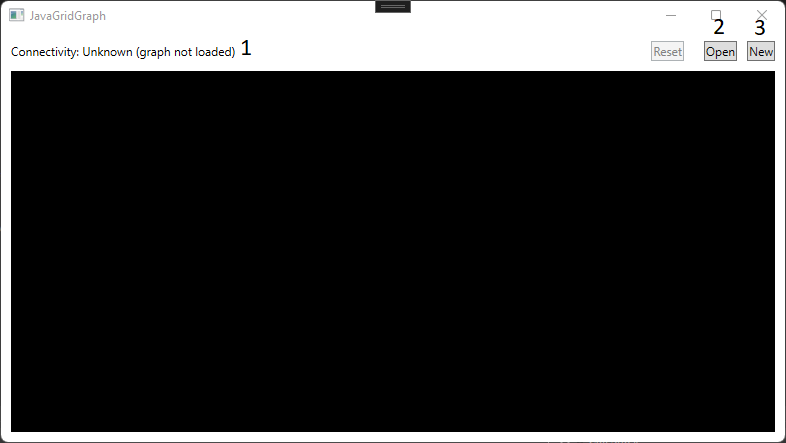
\includegraphics[width=\textwidth]{view1.png}

    \begin{enumerate}
        \item Wynik sprawdzenia spójności grafu. W przypadku gdy graf nie został wczytany, zostanie pokazana informacja o tym że graf nie został wczytany.
        \item Przycisk "Open" otwiera systemowe okno wyboru pliku w celu wybrania pliku zawierającego graf
        \item Przycisk "New" otwiera okno generowania grafu. Więcej informacji w punkcie "Okno generowania grafu".
    \end{enumerate}

    \subsection{Okno generowania grafu}

    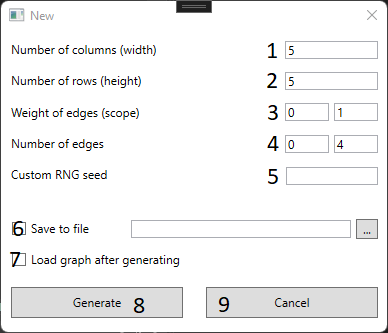
\includegraphics[width=\textwidth]{view2.png}

    \begin{enumerate}
        \item Liczba kolumn (szerokość) grafu. Nie może być mniejsza niż 1.
        \item Liczba wierszy (wysokość) grafu. Nie może być mniejsza niż 1.
        \item Waga krawędzi. Wartość w obu polach nie może być mniejsza od 0, dodatkowo wartość w pierwszym polu (od lewej) musi być mniejsza bądź równa wartości w drugim polu.
        \item Liczba krawędzi wychodzących z pojedyńczego wierzchołka. Wartość w obu polach nie może być mniejsza od 0 i większa od 4, dodatkowo wartość w pierwszym polu (od lewej) musi być mniejsza bądź równa wartości w drugim polu.
        \item Niestandardowe ziarno generatora liczb losowych. Musi być liczbą całkowitą.
        \item Zaznaczenie tego pola spowoduje zapisanie grafu w podanej w polu po prawej lokalizacji. Lokalizację można wybrać także za pomocą przycisku "...". Kliknięcie go spowoduje otworzenie systemowego okna zapisu pliku.
        \item Zaznaczenie tego pola spowoduje wczytanie grafu do programu zaraz po jego wygenerowaniu.
        \item Kliknięcie przycisku spowoduje wygenerowanie grafu o podanych parametrach.
        \item Kliknięcie przycisku spowoduje zamknięcie okna
    \end{enumerate}

    \subsection{Okno główne - po wczytaniu grafu}

    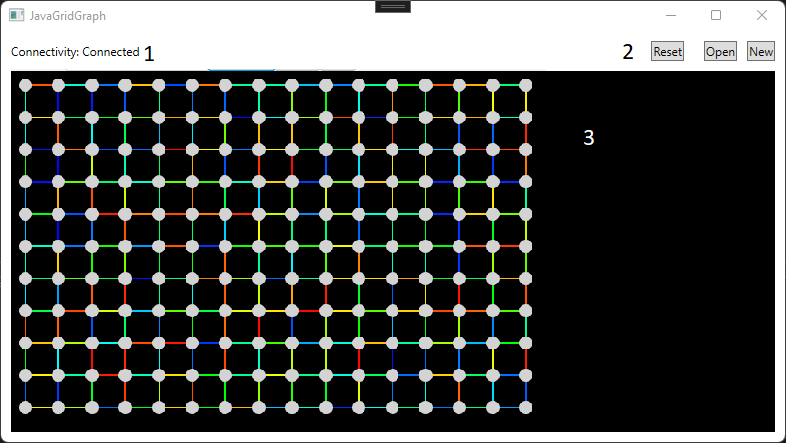
\includegraphics[width=\textwidth]{view3.png}

    \begin{enumerate}
        \item Wynik sprawdzenia spójności grafu. "Connected" - spójny, "Unconnected" - niespójny.
        \item Kliknięcie przycisku spowoduje odznaczenie wszystkich zaznaczonych wierzchołków na grafie.
        \item Pole w którym wyświetlany jest graf. Aby znaleźć najkrótsze ścieżki musimy wybrać wierzchołek $A$ prawym przyciskiem myszy oraz wierzchołki $B_n$ lewym przyciskiem myszy. Po wybraniu wierzchołka $A$ oraz przynajmniej jednego wierzchołka $B$ zostanie narysowana najkrótsza ścieżka od wierzchołka $A$ do wierzchołka $B_n$.
    \end{enumerate}




    \newpage
    \section{Format danych wejściowych i wyjściowych}
    Dane wejściowe i wyjściowe przechowują graf w postaci listy sąsiedztwa. W pierwszej linijce znajdują się dwie liczby, które oznaczają odpowiednio liczbę kolumn i wierszy danego grafu. Każda następna linijka reprezentuje jeden wierzchołek, przy czym wierzchołki numerujemy od 0 od lewej do prawej. Zatem druga linijka w pliku zawiera numery wierzchołków, z którymi połączony jest wierzchołek numer 0, kolejna dotyczy wierzchołka numer 1 itd. Przy każdym numerze wierzchołka po dwukropku podana jest waga krawędzi pomiędzy tymi dwoma wierzchołkami.

    \vspace{1em}

    \noindent
    \textbf{Przykład:}

    \begin{multiconsole}
        2 2

        \hspace*{2em}1 :0.54  2 :0.78

        \hspace*{2em}0 :0.54  3 :0.12

        \hspace*{2em}0 :0.78  3 :0.89

        \hspace*{2em}1 :0.12  2 :0.89
    \end{multiconsole}

    Powyżej przedstawiona jest przykładowa zawartość pliku przechowującego graf. W pierwszej linijce można odczytać, że jest to graf o dwóch kolumnach i dwóch wierszach. W drugiej linijce przedstawiona jest informacja o tym, że wierzchołek numer 0 połączony jest z wierzchołkiem numer 1, a krawędź ta ma wagę 0.54. Istnieje również krawędź pomiędzy wierzchołkiem 0 a 2 o wadze 0.78. W trzeciej linijce znajdują się numery wierzchołków połączonych z wierzchołkiem numer 1 wraz z wagami itd.





    \newpage
    \chapter{Specyfikacja funkcjonalna}

    \newpage
    \section{Diagram klas}

    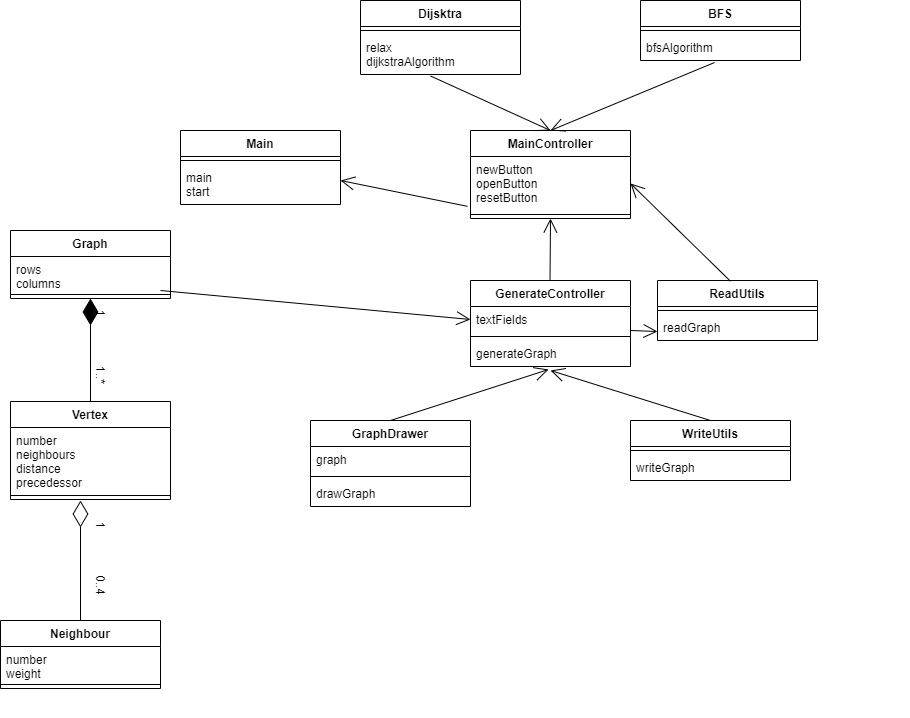
\includegraphics[width=\textwidth]{diagram.png}
\end{document}